\documentclass[11pt,a4paper]{article}
\usepackage[T1]{fontenc}
\usepackage[margin=2.3cm]{geometry}
\usepackage{amsmath,amssymb}
\usepackage{graphicx}
\usepackage[dvipsnames]{xcolor}
\usepackage{enumitem}
\usepackage[colorlinks=true,linkcolor=blue,urlcolor=blue]{hyperref}
\setlength{\parskip}{0.6em}
\setlength{\parindent}{0pt}
\begin{document}

\begin{center}{\LARGE\bfseries opensolarbattery}\\[0.4em]{\large Size a rooftop solar and battery system for a home, one honest simulation at a time.}\\[0.2em]\small PAN IIT OSS explainer \textbullet{} diploma / undergraduate to advanced undergraduate (levels 5-6)\end{center}

\section*{Why this exists}
Sizing a rooftop solar and battery system is a bookkeeping problem about energy in time. This explainer shows how the sun, the household demand, the battery rules and the weather combine into hourly and yearly balances, using only curves, areas and simple rules, so you can build it yourself.

\section*{The end goal}
Size a rooftop solar and battery system for a home. The end goal is a clear, honest sizing method for a home: how big an array and battery meet a reliability target at the lowest cost, and how sure we can be. The same bookkeeping applies to microgrids, water tanks and any storage system. This is an educational model with illustrative costs, not an installation design.

\section*{How the three sessions build up}
\begin{enumerate}[nosep]
\item \textbf{Session 1: A day of sunshine against a day of demand} (Level 1, conceptual interactive model, 60 min).
\item \textbf{Session 2: The hourly balance with a battery} (Level 2, mathematical engineering model, 75 min).
\item \textbf{Session 3: A whole year: reliability and the cost-optimal size} (Level 3, simulation and validation, 90 min).
\end{enumerate}

\section{Session 1: A day of sunshine against a day of demand}

\subsection*{A. Real-world problem}
A neighbour puts a solar array on the roof, yet the evening lights still run on grid power. Why? The sun makes power around noon, but a home uses most of its energy in the morning and the evening. Where the solar curve is above the demand curve there is a surplus nobody can use yet; where it is below, there is a deficit that something else must cover. This session draws both curves and measures the areas. It is an educational model, not an installation design, and nothing here is personal advice.

\subsection*{B. Concept and theory}
Power is the rate of using energy, in kilowatts (kW). Energy is power multiplied by time, in kilowatt-hours (kWh): a 2 kW heater running for 3 hours uses 6 kWh. On a clear day the solar output rises and falls like half a sine wave between sunrise (6 h) and sunset (18 h), so the day's solar energy is the area under that half sine: array rating times 24 divided by pi, about 7.64 kWh per kW. The household demand has a small base load plus a morning and a bigger evening peak. We scale its shape so its area equals the daily energy you choose. Surplus is the area where solar is above demand, deficit the area where demand is above solar, and direct use is the area under the lower of the two curves.

\begin{itemize}[nosep]
\item P\_peak: array rating: output in full sun at noon (kW)
\item s: sun factor: 1 is a clear day, 0.5 a dull day (no unit)
\item P\_pv(t): solar power at time t (kW)
\item P\_load(t): household demand at time t (kW)
\item E: energy: area under a power curve (kWh)
\item t: time of day (hours)
\end{itemize}

\begin{equation*}
P_{pv}(t)=P_{peak}\,s\,\sin\!\left(\frac{\pi (t-6)}{12}\right),\qquad 6\le t\le 18
\end{equation*}

\begin{equation*}
E_{pv}=\int_6^{18} P_{pv}\,dt=P_{peak}\,s\,\frac{24}{\pi}\approx 7.64\,P_{peak}\,s\ \ \mathrm{kWh}
\end{equation*}

\begin{equation*}
E_{surplus}=\int \max\!\big(P_{pv}-P_{load},0\big)dt,\qquad E_{deficit}=\int \max\!\big(P_{load}-P_{pv},0\big)dt
\end{equation*}

\begin{equation*}
E_{direct}=\int \min\!\big(P_{pv},P_{load}\big)dt,\qquad E_{pv}=E_{direct}+E_{surplus},\quad E_{load}=E_{direct}+E_{deficit}
\end{equation*}

\begin{center}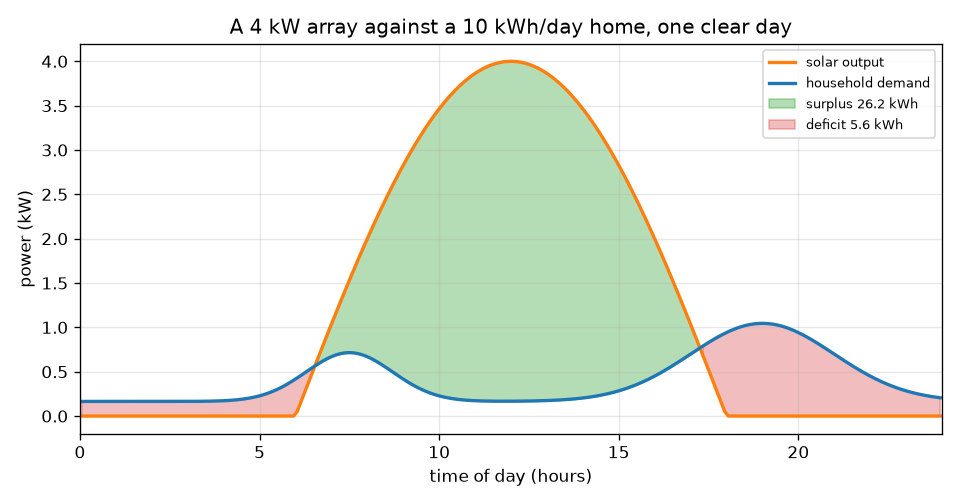
\includegraphics[width=0.85\linewidth]{figures/s01_day_curves.png}\\\small A 4 kW array against a 10 kWh/day home: surplus in green, deficit in red.\end{center}

\subsection*{E. Worked example}
A 4 kW array on a clear day, a home that uses 10 kWh per day. How much solar energy is made? How much is surplus and how much is deficit? Check that the numbers add up.
\begin{enumerate}[nosep]
\item Solar energy = 4 kW x 24 / pi = 4 x 7.639 = 30.56 kWh.
\item From the lesson's area sums: direct use = 4.36 kWh, surplus = 26.20 kWh, deficit = 5.64 kWh.
\item Check the solar side: direct + surplus = 4.36 + 26.20 = 30.56 kWh, which equals the solar energy.
\item Check the demand side: direct + deficit = 4.36 + 5.64 = 10.00 kWh, which equals the demand.
\item Solar share of demand = 4.36 / 10 = 43.6 percent; share of solar used directly = 4.36 / 30.56 = 14.3 percent.
\end{enumerate}
\textbf{Answer.} The array makes 30.56 kWh, three times the demand, yet only 4.36 kWh (43.6 percent of demand) is used directly. The surplus is 26.20 kWh and the deficit is 5.64 kWh.

\subsection*{F. Questions}
\begin{enumerate}[nosep]
\item \textbf{Conceptual.} A home has solar panels that make three times its daily energy on a clear day. Why can it still need the grid every evening?
\item \textbf{Numerical.} A 2 kW array on a dull day (sun factor 0.5) feeds a home that uses 10 kWh per day. How much solar energy is made, and what is the smallest possible grid energy that day?
\item \textbf{Graph and simulation interpretation.} In the second figure the share of solar used directly falls as the array grows, while the share of demand met rises. Explain both trends and say what a battery would change.
\item \textbf{Design and optimisation challenge.} Design: a family wants their solar energy to equal their daily use of 10 kWh on a clear day. What array size is that, and roughly what share of their demand will be met directly by solar? Does this remove their bill?
\end{enumerate}

\section{Session 2: The hourly balance with a battery}

\subsection*{A. Real-world problem}
Session 1 showed that solar alone met less than half of a home's demand. A battery stores the midday surplus and releases it in the evening. But batteries cost money, can only charge and discharge at a limited power, and lose some energy each cycle. How big must the array and the battery be so that the grid supplies only 10 percent of the home's energy on a dull day, and what does each extra kW and kWh add to the cost? All costs here are illustrative units, not market prices, and this is an educational model, not an installation design.

\subsection*{B. Concept and theory}
Work in steps of one hour. In each hour compute the net power: net = solar minus demand. If net is positive the battery charges, limited by its power limit and by the free space; a fraction eta\_c of the energy put in is stored. If net is negative the battery discharges, limited by its power limit and by the stored energy; the house receives eta\_d times the energy taken out of the store. Anything the battery cannot cover is imported from the grid; surplus it cannot absorb is exported. The round-trip efficiency eta is eta\_c times eta\_d, so each way is the square root of eta. The state of charge (SOC) changes by eta\_c x charge - discharge / eta\_d each hour. Self-sufficiency is one minus import divided by demand. The simulation must obey energy conservation.

\begin{itemize}[nosep]
\item P\_pv, P\_load: solar and demand power in an hour (kW)
\item C: usable battery capacity (kWh)
\item P\_max: battery charge and discharge power limit (kW)
\item eta: round-trip efficiency (0.9 means 90 percent) (no unit)
\item SOC: state of charge: energy stored (kWh)
\item SS: self-sufficiency: share of demand not taken from the grid (no unit)
\item cost: illustrative cost: 1000 per kW of array plus 400 per kWh of battery (cost units)
\end{itemize}

\begin{equation*}
\mathrm{net}_h=P_{pv,h}-P_{load,h}\ \ \mathrm{(kW)}
\end{equation*}

\begin{equation*}
\mathrm{charge}_h=\min\!\left(\mathrm{net}_h,\ P_{max},\ \frac{C-SOC_h}{\eta_c\,\Delta t}\right)\ \ (\mathrm{net}_h>0)
\end{equation*}

\begin{equation*}
\mathrm{discharge}_h=\min\!\left(-\mathrm{net}_h,\ P_{max},\ \frac{\eta_d\,SOC_h}{\Delta t}\right)\ \ (\mathrm{net}_h<0)
\end{equation*}

\begin{equation*}
SOC_{h+1}=SOC_h+\eta_c\,\mathrm{charge}_h\Delta t-\frac{\mathrm{discharge}_h\Delta t}{\eta_d},\qquad \eta_c=\eta_d=\sqrt{\eta}
\end{equation*}

\begin{equation*}
E_{pv}+E_{import}=E_{load}+E_{export}+\Delta SOC+E_{losses},\qquad SS=1-\frac{E_{import}}{E_{load}}
\end{equation*}

\begin{center}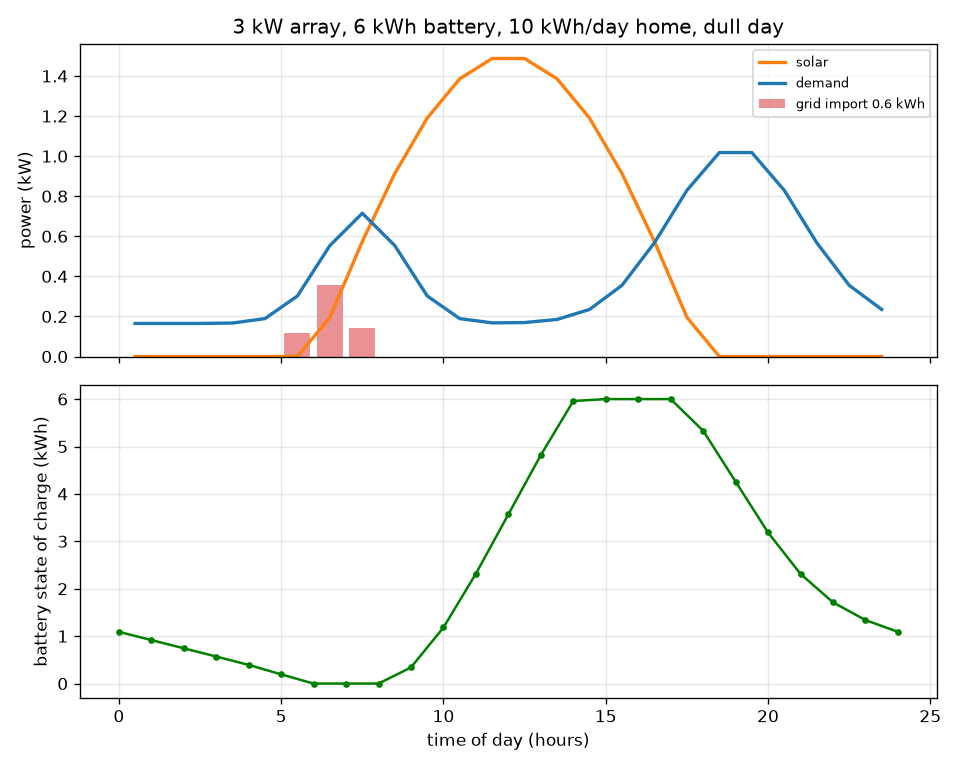
\includegraphics[width=0.85\linewidth]{figures/s02_energy_balance.png}\\\small A dull day for a 3 kW array and 6 kWh battery: hourly balance (top) and state of charge (bottom).\end{center}

\subsection*{E. Worked example}
Part 1 (hand calculation). A battery with round-trip efficiency 0.81 sees a 2 kW surplus for one hour, and later the house draws 1.62 kW from it for one hour. How much is stored and does it empty? Part 2. Use the lesson's search to find the cheapest design for 90 percent self-sufficiency on the dull day.
\begin{enumerate}[nosep]
\item Each way is sqrt(0.81) = 0.9. Surplus hour: charge 2 kW x 1 h = 2 kWh in, stored = 2 x 0.9 = 1.8 kWh.
\item Discharge hour: the house takes 1.62 kWh. The battery must give up 1.62 / 0.9 = 1.8 kWh of stored energy, so it ends empty and no energy is imported.
\item Round trip: 1.62 / 2 = 0.81, which equals eta. The missing 0.38 kWh went to losses.
\item Design search: try array 1 to 8 kW (step 0.5) and battery 0 to 20 kWh (step 1), power limit half the capacity, sun factor 0.5, demand 10 kWh/day, efficiency 0.9.
\item Cheapest design with SS at least 0.9: 3 kW array and 6 kWh battery, SS = 0.938, cost = 1000 x 3 + 400 x 6 = 5400 units. Lower targets cost less: 0.6 needs 2 kW + 3 kWh (3200), 0.8 needs 2.5 kW + 5 kWh (4500).
\end{enumerate}
\textbf{Answer.} Part 1: 1.8 kWh stored, battery ends empty, no import, round trip 0.81. Part 2: 3 kW and 6 kWh, self-sufficiency 0.938, illustrative cost 5400 units.

\subsection*{F. Questions}
\begin{enumerate}[nosep]
\item \textbf{Conceptual.} Why does a lower round-trip efficiency increase the grid import even when the array and battery sizes stay the same?
\item \textbf{Numerical.} A battery with round-trip efficiency 0.64 (0.8 each way) is charged by a 4 kW array while the house uses 1 kW, for one hour. How much energy is stored, and how much can the house later draw from it?
\item \textbf{Graph and simulation interpretation.} On the state-of-charge graph of the 3 kW / 6 kWh design, the battery sits at 6 kWh for several hours in the afternoon. What does that flat top tell you, and would a bigger battery change the import?
\item \textbf{Design and optimisation challenge.} Design: the family accepts 80 percent self-sufficiency instead of 90 on the dull day. Which design is the cheapest, how much is saved, and what is the trade-off?
\end{enumerate}

\section{Session 3: A whole year: reliability and the cost-optimal size}

\subsection*{A. Real-world problem}
A design that works on one dull day can still fail in a cloudy fortnight in winter. A sizing decision has to hold up over a whole year of changing day length, clouds and demand. How big must the array and battery be so that the grid supplies no more than 10 percent of the home's energy over a year? And why does adding battery capacity not necessarily solve every problem caused by an undersized solar array? Costs are illustrative units, not market prices; the model is educational, not an installation design, and nothing here is personal or financial advice.

\subsection*{B. Concept and theory}
We build the year from three ingredients. Clear-sky solar: day length D(d) and noon strength A(d) follow the seasons, so a clear day gives A x 2D / pi kWh per kW. Clouds: each day gets a cloud cover B between 0 and 1, from a seeded, correlated random sequence (clouds last a few days), and the day's clearness is K = 1 - 0.9 c B, where c is the cloudiness setting. Demand: the daily energy comes from a bill (or a default seasonal pattern), with a seeded 10 percent day-to-day wobble. The battery rules are those of Session 2, carried through all 8760 hours without a reset. Reliability is the energy reliability R = 1 - unmet / demand, where unmet is the grid import, and the loss-of-load hours (LOLH) count the hours in which import occurs. Because no battery can create energy, R can never exceed solar energy divided by demand: this is the ceiling that an undersized array imposes. We validate the code against exact rules, then search a grid of (array, battery) designs and keep the Pareto front: designs for which no other design is both cheaper and more reliable.

\begin{itemize}[nosep]
\item d: day of the year (0 to 364) (days)
\item D(d), A(d): day length and noon strength for day d (hours, no unit)
\item c: cloudiness setting, 0 (cloudless) to 1 (very cloudy) (no unit)
\item B, K: daily cloud cover and clearness (K multiplies solar) (no unit)
\item R: energy reliability = 1 - unmet / demand (no unit)
\item LOLH: loss-of-load hours: hours with grid import above 0.001 kW (hours)
\item seed: number that makes the random year repeatable (no unit)
\end{itemize}

\begin{equation*}
D(d)=12+2.5\sin\!\frac{2\pi(d-80)}{365},\qquad A(d)=0.85+0.10\sin\!\frac{2\pi(d-80)}{365}
\end{equation*}

\begin{equation*}
P_{pv}(d,t)=P_{peak}\,K_d\,A(d)\sin\!\frac{\pi (t-t_{rise})}{D(d)},\qquad E_{clear}(d)=P_{peak}A(d)\frac{2D(d)}{\pi}
\end{equation*}

\begin{equation*}
K_d=1-0.9\,c\,B_d,\qquad B_d=\Phi(z_d),\ \ z_d=0.6\,z_{d-1}+0.8\,e_d,\ \ e_d\sim N(0,1)
\end{equation*}

\begin{equation*}
R=1-\frac{E_{import}}{E_{load}},\qquad R\le \min\!\left(1,\frac{E_{pv}}{E_{load}}\right)
\end{equation*}

\begin{equation*}
E_{pv}+E_{import}=E_{load}+E_{export}+\Delta SOC+E_{losses}
\end{equation*}

\begin{center}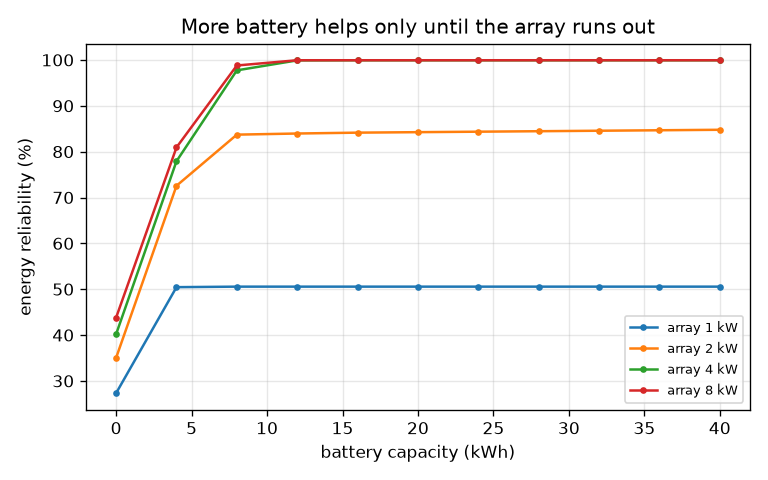
\includegraphics[width=0.85\linewidth]{figures/s03_battery_vs_array.png}\\\small Reliability against battery capacity: small arrays stall below the ceiling.\end{center}

\subsection*{E. Worked example}
Part 1 (analytic reference). Check the hourly clear-sky model against the exact formula A x 2D / pi summed over the year. Part 2. Find the cost-optimal design for R at least 0.9 with cloudiness 0.5, seed 1, demand 10 kWh per day on average (3642 kWh in the simulated year), and check how robust it is.
\begin{enumerate}[nosep]
\item Sum over the 365 days of A(d) x 2D(d) / pi: 2399 kWh per kW. The hourly simulator adds 365 x 24 hourly values: 2401 kWh per kW. They agree to better than 0.1 percent.
\item With clouds (cloudiness 0.5, seed 1) the year gives 1936 kWh per kW: mean clearness 0.805 against the expected 1 - 0.45 x 0.5 = 0.775 (one random year differs from the average).
\item Check the energy conservation: solar + import - (demand + export + change in storage + losses) = 0 within rounding for the whole year.
\item Search 20 array sizes (0.5 to 10 kW) x 25 battery sizes (0 to 24 kWh) = 500 designs. The cheapest with R at least 0.9 is 2.5 kW + 7 kWh: R = 0.902, loss-of-load hours 1117, cost 1000 x 2.5 + 400 x 7 = 5300 units.
\item Robustness: run the same design on 100 other random years. It reaches R at least 0.9 in only 15 of 100, and its 5th-percentile reliability is 0.884. The design 3 kW + 8 kWh (cost 6200) reaches it in all 100 years (5th percentile 0.938).
\end{enumerate}
\textbf{Answer.} Hourly clear-sky energy 2401 kWh per kW matches the analytic 2399 kWh per kW. The cheapest design for one simulated year is 2.5 kW + 7 kWh (cost 5300, R = 0.902), but it is only lucky in that year; 3 kW + 8 kWh (cost 6200) is reliable in all 100 test years.

\subsection*{F. Questions}
\begin{enumerate}[nosep]
\item \textbf{Conceptual.} Why does increasing the battery capacity not necessarily solve every problem caused by an undersized solar array?
\item \textbf{Numerical.} A 4 kW array and an 8 kWh battery give reliability 0.977 for a home with 3642 kWh of demand in the simulated year. How much energy did the home import? If the demand is 30 percent higher, reliability falls to 0.901: how many more kWh were imported?
\item \textbf{Graph and simulation interpretation.} In the sensitivity results for the 4 kW / 8 kWh design, reliability is 0.982 at cloudiness 0, 0.977 at 0.5, 0.956 at 0.75 and 0.897 at 1.0. What do the loss-of-load hours (188, 218, 477, 1028) add?
\item \textbf{Design and optimisation challenge.} Design: choose the array and battery for 95 percent reliability and justify your choice against the Pareto front. Would you pick the single-year optimum or something larger?
\end{enumerate}

\section{Real-world mini-project}
\textbf{Size a system from your own electricity bill.} Take 12 monthly electricity readings in kWh from a household (your own, a relative's, or invent a realistic set). Use \texttt{monthly\_to\_daily} and \texttt{size\_from\_bill} from Session 3 to find the cheapest array and battery for 90 percent energy reliability, then test it against a cloudier year. Treat the output as a classroom estimate: it is not an installation design, and the costs are illustrative units.

\section{The path ahead}
\begin{enumerate}[nosep]
\item \textbf{Session 4: Robust sizing over many weather years.} A search that evaluates every candidate design over many seeds and keeps a design meeting the target in most of them.
\item \textbf{Session 5: A smarter search.} An optimiser that replaces the 500-design grid.
\item \textbf{Session 6: Backup for a power cut.} A critical-load model and an outage scenario in the yearly simulator.
\item \textbf{Session 7: Real weather and real demand.} A loader for an hourly irradiance file and a smart-meter file, with the same battery code.
\item \textbf{Session 8: Reproduce the Target animation.} A 24-hour animation of one simulated day with flow arrows and a battery level, plus the cost-versus-reliability chart.
\end{enumerate}

\section{Answers and hints}

\subsection*{Session 1}
\begin{enumerate}[nosep]
\item \textbf{Conceptual.} Hint: Compare when solar is available with when demand is highest. Solution: Energy made and energy needed are measured over the whole day, but they do not happen at the same time. Solar output is near zero in the evening when demand peaks, and large at midday when demand is low, so most of the solar energy is surplus. Without storage the surplus cannot be moved to the evening, so the deficit still comes from the grid.
\item \textbf{Numerical.} Hint: Solar energy = P\_peak x s x 24 / pi. The deficit can never be smaller than demand minus solar energy. Solution: Solar energy = 2 x 0.5 x 7.639 = 7.64 kWh. Even if every kWh were used perfectly, the home still needs at least 10 - 7.64 = 2.36 kWh from elsewhere. In practice the deficit is larger because the timing does not match. Units: kWh.
\item \textbf{Graph and simulation interpretation.} Hint: Where does the extra energy of a bigger array arrive in the day? Solution: A bigger array adds output mostly at midday, when demand is already met, so the extra energy becomes surplus: the share of solar used falls (41.4 percent at 1 kW to 7.5 percent at 8 kW). The share of demand met rises only slowly (31.6 to 45.8 percent) because evening demand is still uncovered. A battery would store the midday surplus and release it in the evening, raising both shares.
\item \textbf{Design and optimisation challenge.} Hint: Use E = P\_peak x 24 / pi, then compare with the sizes in the table printed by the lesson. Solution: P\_peak = 10 / 7.639 = 1.31 kW. From the printed table, 1 kW meets 31.6 percent of demand directly and 2 kW meets 39.1 percent, so 1.31 kW is roughly a third. The bill is not removed: two thirds of the demand still comes from the grid at that moment, even though the day's totals match. Trade-off: a bigger array raises the share only slowly without storage, and a clear day is the best case.
\end{enumerate}

\subsection*{Session 2}
\begin{enumerate}[nosep]
\item \textbf{Conceptual.} Hint: Follow 1 kWh of surplus into the battery and out again. Solution: Every kWh of surplus that goes through the battery comes back as only eta kWh, so part of the stored solar energy is lost as heat. The evening deficit then needs extra grid energy to make up the difference. For the 3 kW / 6 kWh design on the dull day the grid import rises from 0.31 kWh at eta = 1.0 to 0.62 kWh at 0.9 and 0.94 kWh at 0.8.
\item \textbf{Numerical.} Hint: Net surplus = 3 kW for 1 h. Stored = eta\_c x energy. Output = eta\_d x stored. Solution: Surplus energy = 3 kW x 1 h = 3 kWh (assuming the power limit and capacity allow it). Stored = 0.8 x 3 = 2.4 kWh. The house can draw 0.8 x 2.4 = 1.92 kWh = 0.64 x 3. Sanity check: the output is smaller than the input, and 1.92 / 3 = 0.64 = eta.
\item \textbf{Graph and simulation interpretation.} Hint: What happens to surplus when the battery is full? And when is the import actually happening? Solution: A flat top means the battery is full and surplus solar is exported (1.48 kWh that day), so charging is limited by capacity. A bigger battery would store that surplus, but the imports are in the early morning (0.62 kWh), when the battery is empty after the night. Extra capacity helps only if the array makes enough surplus to fill it; here a larger array or a better-kept charge matters more for the morning gap.
\item \textbf{Design and optimisation challenge.} Hint: Use cheapest\_design(0.8) and cost(). Compare with the 90 percent design. Solution: cheapest\_design(0.8) gives 2.5 kW and 5 kWh, SS = 0.818, cost 4500 units, against 5400 for the 90 percent design: a saving of 900 units (17 percent) but 12 percentage points less of the demand met without the grid. Assumptions: one repeated dull day, illustrative costs. A real design would also need the whole year, which Session 3 does.
\end{enumerate}

\subsection*{Session 3}
\begin{enumerate}[nosep]
\item \textbf{Conceptual.} Hint: Compare the energy the array makes in a year with the energy the home uses, and think about winter weeks. Solution: A battery only moves energy in time; it cannot create it. If the array makes less energy than the home needs, no battery can close the gap: reliability is capped at solar energy divided by demand (0.531 for the 1 kW array in the simulated year, and the 1 kW array stays at 50.6 percent with 8, 16 or 40 kWh). Even when the yearly total is enough (the 2 kW array reaches only about 85 percent), cloudy winter weeks leave the battery empty, and an extra kWh of capacity is not filled because there is no surplus to fill it. The array must grow first.
\item \textbf{Numerical.} Hint: Import = (1 - R) x demand. New demand = 1.3 x 3642. Solution: Import = (1 - 0.977) x 3642 = 83 kWh (the code prints 82.7 kWh). With demand scaled by 1.3 the demand is 4735 kWh and the import is (1 - 0.901) x 4735 = 469 kWh, so about 386 kWh more. Units: kWh. Sanity check: demand rose 30 percent but import rose more than five times, because the extra evening demand finds the battery empty.
\item \textbf{Graph and simulation interpretation.} Hint: Compare how quickly each measure changes. Solution: Reliability measures the share of energy that is unmet, while loss-of-load hours count how often the home needs the grid. Between cloudiness 0.5 and 0.75, reliability falls only 2.1 percentage points but the hours of import more than double (218 to 477), and at cloudiness 1.0 the grid is needed for 1028 hours (about 12 percent of the year). The change is gentle at first and steep at the cloudy end: a design can look fine on energy and still involve many hours of dependence.
\item \textbf{Design and optimisation challenge.} Hint: Use cheapest(designs, 0.95), then test the design on other seeds with pv\_unit\_year(0.5, seed). Solution: The single-year optimum for R at least 0.95 is 3 kW + 8 kWh (R = 0.953, cost 6200). Because one year is one sample of the weather, test it on other seeds: a design sitting exactly at the target will miss it in many years. Choose a margin: for example 3.5 kW + 9 kWh, then check the 5th-percentile reliability over 100 years. Trade-off: each step along the Pareto front buys a smaller reliability gain for a larger cost (4 kW + 9 kWh costs 7600 for R = 0.994), so the choice depends on how a failure is valued. This is an illustrative classroom model, not a design.
\end{enumerate}

\section{How to join}
Read \texttt{CONTRIBUTING.md} in the repository, then pick an issue labelled \texttt{good first issue}. Repository: \url{https://github.com/KrunalPanchal1995/pan-iit-oss/tree/main/opensolarbattery}

\end{document}
